\section{Überblick der Assoziationsalgorithmen}

Die \gls{Assoziation} ist elementar für \gls{MOT} Systeme. Sie verknüpft die \gls{Detektion}[en] zu \gls{Trajektorie}[n]. Diese Aufgabe wird von sogenannten \gls{Assoziation}[salgorithmen] erledigt. Im folgenden werden zwei Algorithmen vorgestellt, welche im Rahmen dieser Arbeit auf ihre Eignung für die Anwendung in einer automatischen \glsdisp{Klassifikation}{Verhaltensklassifikation} untersucht wurden. Das genau diese beiden Algorithmen betrachtet werden, ist mit der Einfachheit ihrer Integration zu begründen und mit der Verfügbarkeit als Open Source Code. 


\subsection{SORT - Simple Online and Realtime Tracking} \label{sec:MOT SORT}

Wie der Name vermuten lässt ist \acrshort{SORT} ein \gls{Online Tracking} Algorithmus (\autoref{sec:MOT Verarbeitungsverfahren}), welcher speziell auf die Echtzeitverarbeitung ausgelegt ist. Der Algorithmus wird in \cite{Bewley.2016} beschrieben. Aufgrund seiner Einfachheit und Effizienz wird \acrshort{SORT} in einer Vielzahl von Anwendungsfällen benutzt \cite{Chen.2023, Maher.2018, Fedorov.2019}. \par

\acrshort{SORT} benutzt eine Zustandsschätzung mittels Kalman-Filter \cite{Kalman.1960}. Damit wird geschätzt wie sich die Position eines Objektes von einem \gls{Frame} in das nächste verändert. Dies geschieht, indem die Geschwindigkeit als konstant angenommen wird und die Bewegung als linearer Verlauf. Ebenfalls wird die Dimension der \gls{Bounding Box} des Objekts geschätzt. Die Schätzung ist die erwartete Position und Dimension für die \gls{Detektion} des Objekts im folgenden \gls{Frame}. Diese Erwartungswerte werden mit \gls{Detektion}[en] zugeordnet. Dies geschieht indem zunächst die Ähnlichkeit von der \gls{Detektion} und der Schätzung bestimmt wird. Als Maß für die Ähnlichkeit wird die \glsdisp{IoU}{Intersection over Union (\(IoU\))} benutzt  \cite{Bewley.2016}. Die \(\gls{IoU}\) ist der Quotient aus der Schnittmenge und der Vereinigungsmenge zweier Mengen. Im Bezug auf den \acrshort{SORT} Algorithmus bezieht sich die \(\gls{IoU}\) auf die Fläche der \gls{Bounding Box} der \gls{Detektion} und der Schätzung. Die \autoref{fig:IoU} visualisiert die \(\gls{IoU}\) und die \autoref{eq:IoU} zeigt die Berechnung \cite{Rezatofighi.2019}. 

\begin{equation}
    \label{eq:IoU}
    \frac{A \cap B}{A \cup B} = IoU\
\end{equation}
\begin{wrapfigure}{r}{0.4\textwidth}
    \begin{center}
        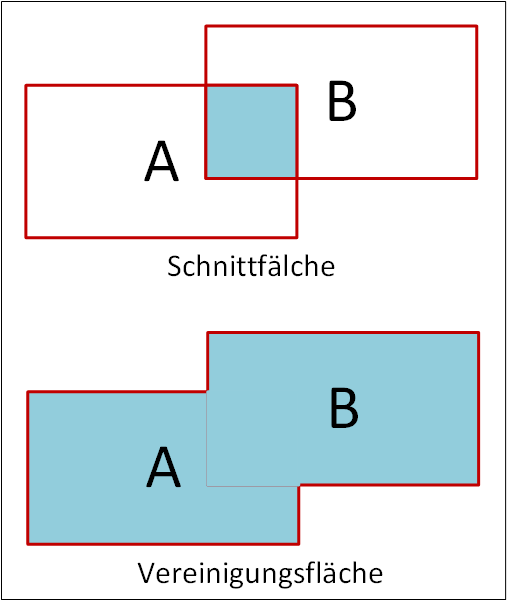
\includegraphics[width=0.4\textwidth]{img/Grafiken/IoU.png}
        \caption[Schnittfläche und Vereinigungsfläche zweier Bounding Boxen.]{Schnittfläche und Vereinigungsfläche zweier \gls{Bounding Box}[en].}
        \label{fig:IoU}
    \end{center}
\end{wrapfigure}

In der Praxis kommt es dazu, dass mehrere für die Zuordnung von einer Schätzung mehrere \gls{Detektion}[en] in Frage kommen. Um direkt \gls{Detektion}[en] ausschließen zu können kann ein Schwellwert für die \(\gls{IoU}\) definiert werden \(\gls{IoU}_{min}\), welcher mindestens erreicht seien muss. Für jede Schätzung existiert eine Menge an \gls{Detektion}[en] aus denen die beste Zuordnung auszuwählen ist. Dieses Zuordnungsproblem löst der \acrshort{SORT} Algorithmus mit der Ungarischen Methode \cite{Kuhn.1955}. Diese sucht nach der Zuordnung, welche die globale \(\gls{IoU}\) des betrachteten \gls{Frame}[s] maximiert. Somit ist die \gls{Assoziation} für dieses \gls{Frame} gelöst. Die Zuordnungen aktualierieren den Kalman-Filter für die nächsten Schätzungen \cite{Bewley.2016}. \par

\acrshort{SORT} ist in der Lage mit kurzzeitigen Verdeckungen oder \gls{Detektion}[saussetzern] umzugehen. Ist in einem \gls{Frame} keine Zuordnung von einem Objekt möglich, dann wird die Annahme der linearen Bewegung mit konstanter Geschwindigkeit für das folgende Bild fortgesetzt. Dort wird dann versucht das Objekt zu reidentifizieren. Lies sich das Objekt für mehrere aufeinander folgende \gls{Frame}[s] nicht zuordnen, wird die \gls{Assoziation} zu dieser \gls{Trajektorie} abgebrochen. Die Anzahl der \gls{Frame}[s] die ein Objekt unauffindbar bleiben darf ist einstellbar \cite{Bewley.2016}.\par

Als neue \gls{Trajektorie} kommen alle \gls{Detektion}[en] infrage, welche unterhalb \(\gls{IoU}_{min}\) liegen. Für diese \gls{Detektion}[en] wird ein Schätzer initialisiert. Wenn für diese \gls{Detektion} in den folgenden Bildern Zuordnungen gefunden werden können, dann wird eine neue \gls{Trajektorie} initialisiert. Ist dies nicht möglich, so wird die \gls{Trajektorie} verworfen. Die Anzahl der notwendigen \gls{Frame}[s] bis zur Initialisierung lässt sich einstellen \cite{Bewley.2016}.

\subsection{Crocker-Grier Linking Algorithmus} \label{sec:MOT CrockGrier}
Der Crocker-Grier Linking Algorithmus ist auf das Tracking von Partikeln in der Videomikroskopie ausgelegt. Der Algorithmus wird in \cite{Crocker.1996} vorgestellt als Teil verschiedener Bildverarbeitungsmethoden speziell für die Videomikroskopie. Er wird in dieser Arbeit betrachtet, da zuvor entwickelte Anwendungen im \acrshort{OptiLiMa}-Projekt diesen verwenden. Grund dafür ist vor allem die einfache Integrierbarkeit, da die \gls{Python}-\gls{Bibliothek} \cite{Allan.2023} den Crocker-Grier Linking Algorithmus implementiert hat.\par

Die Bewegung von Partikeln in einem Medium ist zufällig und lässt sich stochastisch Beschreiben. Dieses Phänomen beschreibt die \gls{Brownsche Bewegung} \cite{Nelson.1972}. Demnach lässt sich die Wahrscheinlichkeit, dass ein Partikel in einer bestimmten Zeit \(t\) eine Distanz \(\delta\) zurücklegt berechnen \cite{Crocker.1996}. Der Algorithmus nutzt dies als zugrundeliegende Annahme über die Bewegung der zu \glsdisp{Assoziation}{assoziierenden} Objekte. Um ein Objekt aus einem \gls{Frame} mir einer \gls{Detektion} im folgenden \gls{Frame} zu \glsdisp{Assoziation}{assoziieren}, berechnet der Algorithmus die Wahrscheinlichkeiten für die möglichen Bewegungen. Die möglichen Bewegungen sind in diesem Fall die \gls{Detektion}[en], welche für eine \gls{Assoziation} in frage kommen. Die Wahrscheinlichkeit wird anhand der Distanz zwischen der letzten bekannten Position des Objekts und der Position der jeweiligen \gls{Detektion} berechnet. Verarbeitet werden können dabei nur Punkte. Liegen die \gls{Detektion}[en] als \gls{Bounding Box}[en] vor, eignet sich der Mittelpunkt, um den Algorithmus anzuwenden. Werden mehrere Partikel beobachtet, dann lässt sich aus den einzelnen zurückgelegten Distanzen eine Gesamtwahrscheinlichkeit für die kollektive Bewegung ermitteln \cite{Crocker.1996}. Um mehrere Objekte zu \glsdisp{Assoziation}{assoziieren}, versucht der Algorithmus die Zuordnung zu finden, welche die Gesamtwahrscheinlichkeit maximiert. \par

Dies ist die prinzipielle Idee, die der Crocker-Grier Linking Algorithmus verfolgt. Jedoch werden einige Abänderungen getätigt, um den Rechenaufwand zu reduzieren. Um die Gesamtwahrscheinlichkeit über alle möglichen \gls{Assoziation}[en] zu berechnen und zu maximieren ist es notwendig, für jedes Objekt auch jede \gls{Detektion} in Erwägung zu ziehen. Aus diesem Grund wird eine maximale Distanz \(l\) eingeführt, welche die Objekte zwischen zwei \gls{Frame}[s] zurücklegen können. \(l\) ist vom Anwender zu bestimmen, da es von der jeweiligen Situation abhängt. Im Idealfall kommt für jedes Objekt dann nur noch eine \gls{Detektion} in frage. Es kann jedoch auch vorkommen, dass sich Netzwerke bilden von mehreren Objekten und \gls{Detektion}[en], wenn eine \gls{Detektion} näher als \(l\) zu mehreren Objekten liegt. In diesem Fall wird die maximale Gesamtwahrscheinlichkeit für dieses Netzwerk gesucht, um das \gls{Assoziation}[sproblem] zu lösen \cite{Crocker.1996}. \par

Sind in einem Netzwerk mehr \gls{Detektion}[en] als Objekte vorhanden, dann initialisiert der Algorithmus diese als neue \gls{Trajektorie}[n]. Kommt es in einem Netzwerk dazu, dass mehr Objekte vorhanden sind, als \gls{Detektion}[en] kann das \gls{Assoziation}[sproblem] nicht vollständig gelöst werden. Dazu führt der Algorithmus verlorene Objekte ein. Dies kann z.B. durch Verdeckungen oder falsch negative \gls{Detektion}[en] verursacht werden. Um ein Netzwerk zu \glsdisp{Assoziation}{assoziieren} werden so viel verlorene Objekte angenommen damit die Anzahl der Objekte gleich der Anzahl der \gls{Detektion}[en] ist. Anschließend kann das Netzwerk gelöst werden. Objekte die mit einem verlorenen Objekt \glsdisp{Assoziation}{assoziiert} werden, können in folgenden \gls{Frame}[s] wieder zugeordnet werden. Dies ist möglich, da der Algorithmus die Distanz \(l\) annimmt für ein \gls{Frame} indem ein Objekt verloren ist, um im folgenden \gls{Frame} dann mit einem vergrößerten Radius nach möglichen \gls{Assoziation}[en] sucht \cite{Crocker.1996}. \par 

Der Crocker-Grier Linking Algorithmus bekommt Probleme, wenn der Abstand zwischen den Objekten kleiner ist als \(l\). In diesem Fall kommt es dazu, dass die Suche nach der Maximalen Gesamtwahrscheinlichkeit nicht zu einer korrekte Lösung des \gls{Assoziation}[sproblems] führt. \gls{Assoziation}[s]fehler sind die folge. Ebenfalls sind große Netzwerke die folge, was zu einer erhöhten Rechenzeit führt \cite{Crocker.1996}. \par

Die \gls{Python}-\gls{Bibliothek} \cite{Allan.2023} ergänzt den Algorithmus, um einig Funktionen. Hier lässt sich die Anzahl der \gls{Frame}[s] die ein Objekt verloren seien darf begrenzen. Ist ein Objekt länger nicht \glsdisp{Assoziation}{assoziierbar}, wird die \gls{Trajektorie} abgebrochen. Ebenfalls gibt es die Möglichkeit die größe der Netzwerke zu beschränken, um den Rechenaufwand zu kontrollieren. Dies wird möglich in dem \(l\) für jedes \gls{Frame} adaptiv ermittelt wird. Für \(l\) wird ein Startwert gesetzt, dieser wird Schrittweise verkleinert bis alle Netzwerke unterhalb einer bestimmten Größe liegen. \par

Prinzipiell ist der Crocker-Grier Linking Algorithmus ein \gls{Online Tracking} Algorithmus, da er die \gls{Assoziation}[en] nur Basis des aktuellen \gls{Frame}[s] und vergangener \gls{Frame}[s] macht. In \cite{Allan.2023} ist der Algorithmus jedoch so Implementiert, dass nur eine Verarbeitung im Stapel möglich ist (\autoref{sec:MOT Verarbeitungsverfahren}). 

